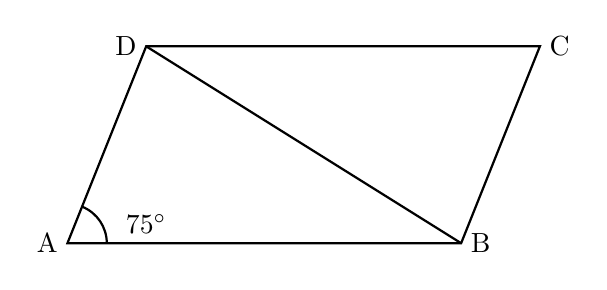
\begin{tikzpicture}[scale=1]

    % Define the coordinates for the parallelogram
    % Base AB is horizontal, D is shifted right to create the acute angle at A
    \coordinate (A) at (0,0);
    \coordinate (B) at (5,0);
    \coordinate (C) at (6,2.5);
    \coordinate (D) at (1,2.5);

    % Draw the boundary of the parallelogram ABCD
    \draw[thick] (A) -- (B) -- (C) -- (D) -- cycle;

    % Draw the diagonal segment from D to B
    \draw[thick] (D) -- (B);

    % Draw the angle arc at vertex A
    % The arc goes from the base (0 degrees) to the line AD (approx 68.2 degrees)
    \draw[thick] (0.5,0) arc (0:68.2:0.5);

    % Add the angle measurement label exactly where it appears
    \node at (1.0, 0.25) {$75^\circ$};

    % Add the labels for the vertices
    \node[left] at (A) {A};
    \node[right] at (B) {B};
    \node[right] at (C) {C};
    \node[left] at (D) {D};

\end{tikzpicture}